\chapter{Resultados Preliminares}

En el presente capítulo se muestran resultados preliminares de la investigación.
Estos resultados se obtuvieron siguiendo la propuesta descrita en el anterior capítulo, pero llegando solo hasta la optimización continua.
Además, los experimentos se realizaron solo con un \emph{bend} utilizando un único algoritmo: CMA-ES.
Con las anteriores restricciones se realizaron tres experimentos.


\section{Experimento 1}

Como primer experimento se comenzó configurando un \emph{bend} con las características descritas en la figura \ref{fig:dimensiones-bend}.
Luego, se procedió a realizar la optimización.
Para la optimización continua se limitó la cantidad de simulaciones a 5000 y para cada una de las 5 etapas de la optimización discreta se limitó en 5000 simulaciones.

\begin{figure}[ht]
  \centering
  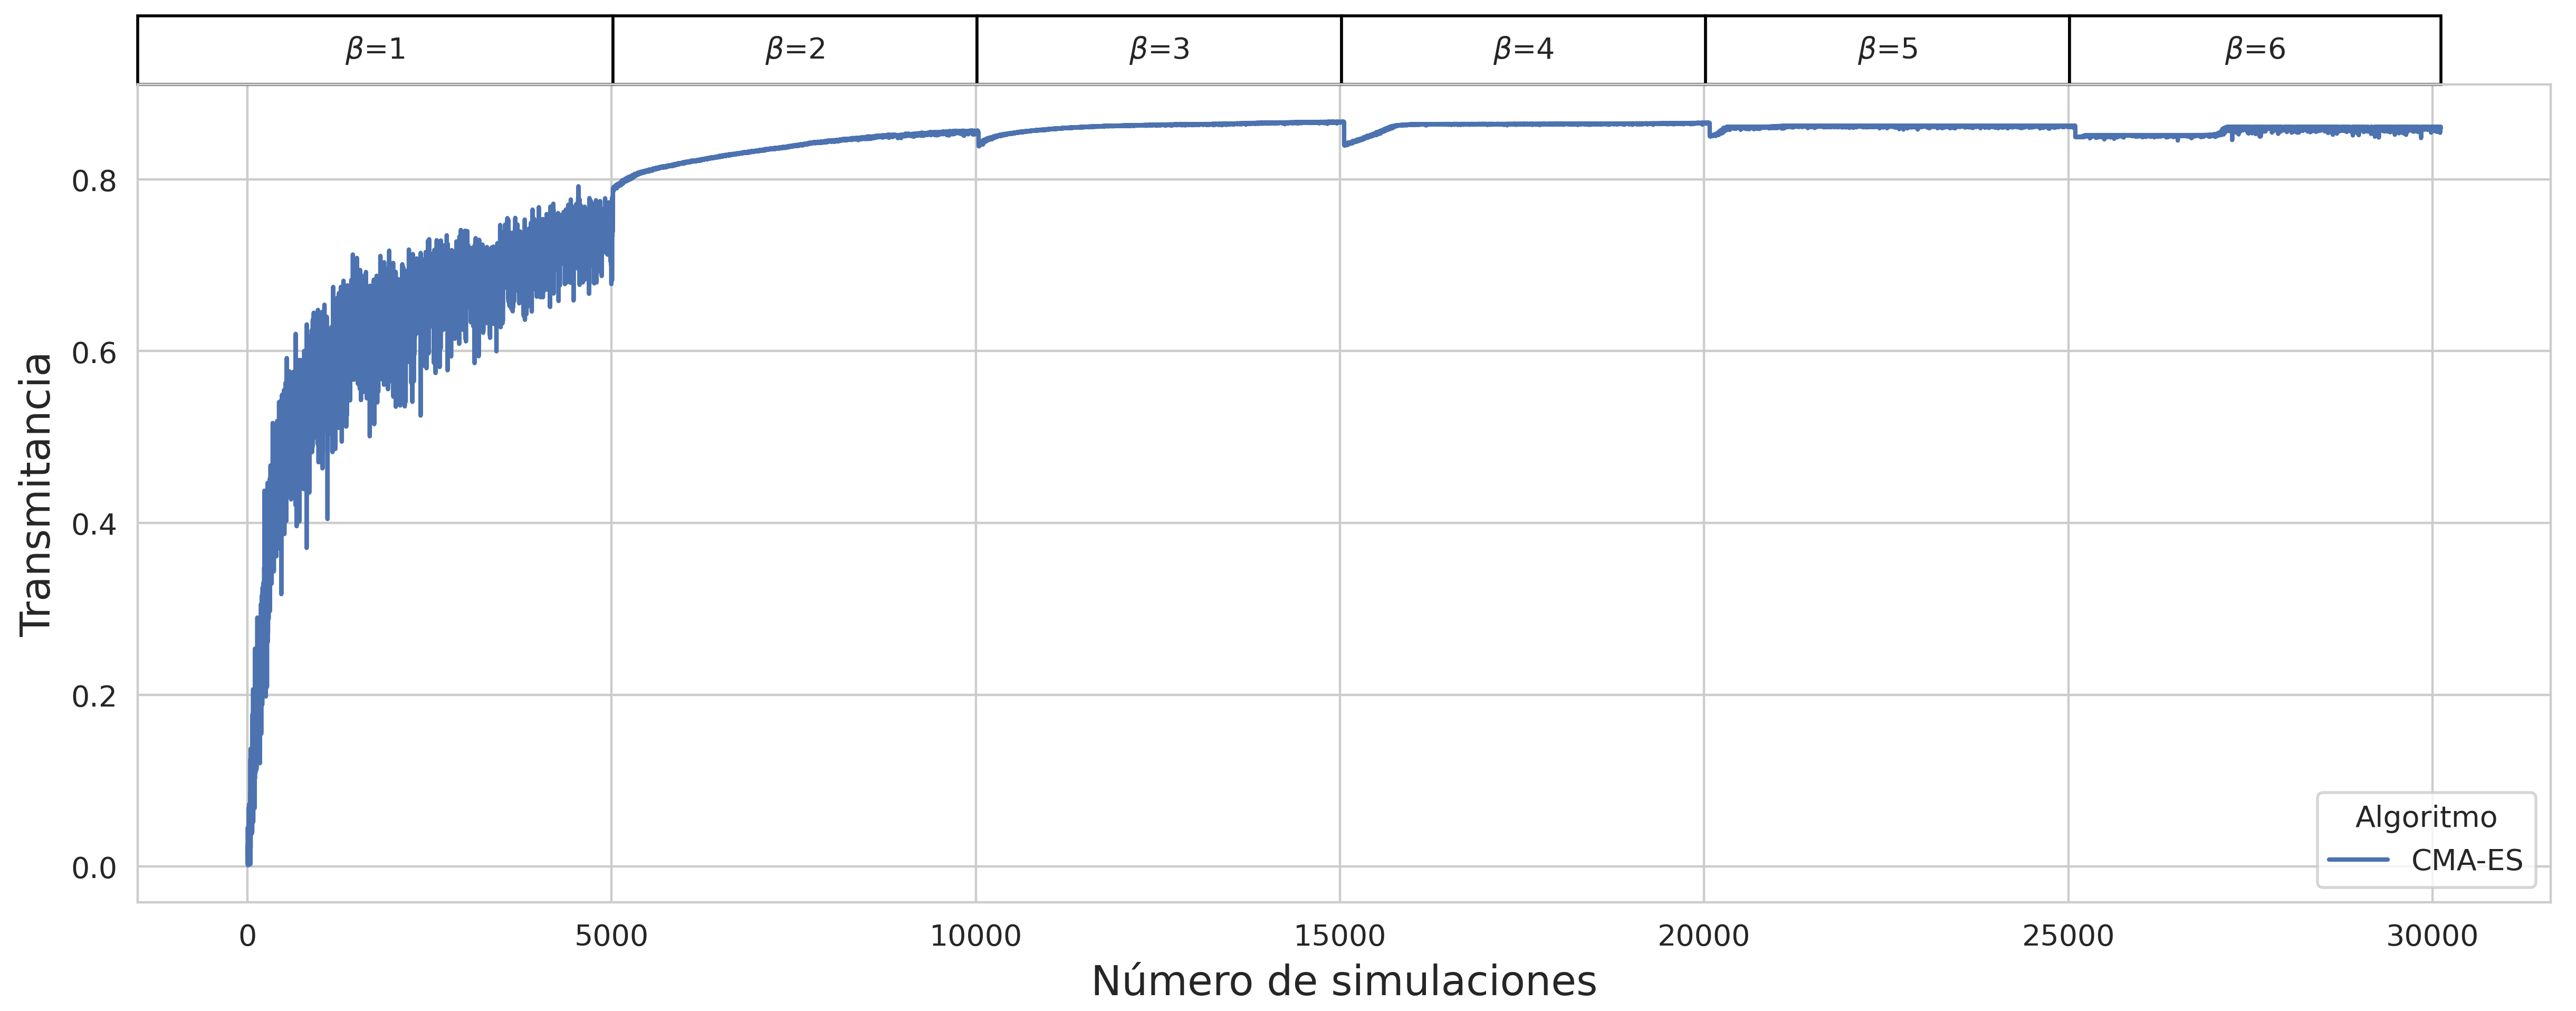
\includegraphics[width=\textwidth]{image/results/iterations_v1.png}
  \caption{Gráfica del número de simulaciones vs transmitancia producto de optimizar un \emph{bend} usando CMA-ES en el experimento 1.}
  \label{fig:iterations-v1}
\end{figure}

En la figura \ref{fig:iterations-v1} se muestra la transmitancia de cada uno de los diseños evaluados.
Podemos observar que en la etapa de la optimización continua, $\beta = 1$, es cuanto mayor crecimiento se logra.
Luego, en los distintos pasos dentro de la optimización discreta $(\beta = 2, 3, 4, 5, 6)$ el crecimiento es más lento.
Sin embargo, es destacable el hecho que aún al incrementar el valor de $\beta$, la simulación sigue logrando explorar diseños con valores de transmitancia similares.
Para lograr esto se comenzó ejecutando el algoritmo con un valor de $\sigma = 0.3$ en la optimización continua y luego se uso $\sigma = 0.01$ en la optimización discreta.


En total el experimento duró 24 horas con 30 minutos y en promedio cada simulación tomó 2.788 segundos.
Esto se debió a que se utilizó una resolución de 100 $nm$.
Pero, como el \emph{bend} que definimos utilizaba un tamaño de píxel de $60 nm$, las simulaciones no estaban logrando simular de forma correcta todos los detalles de los diseños.

\begin{figure}
  \centering
  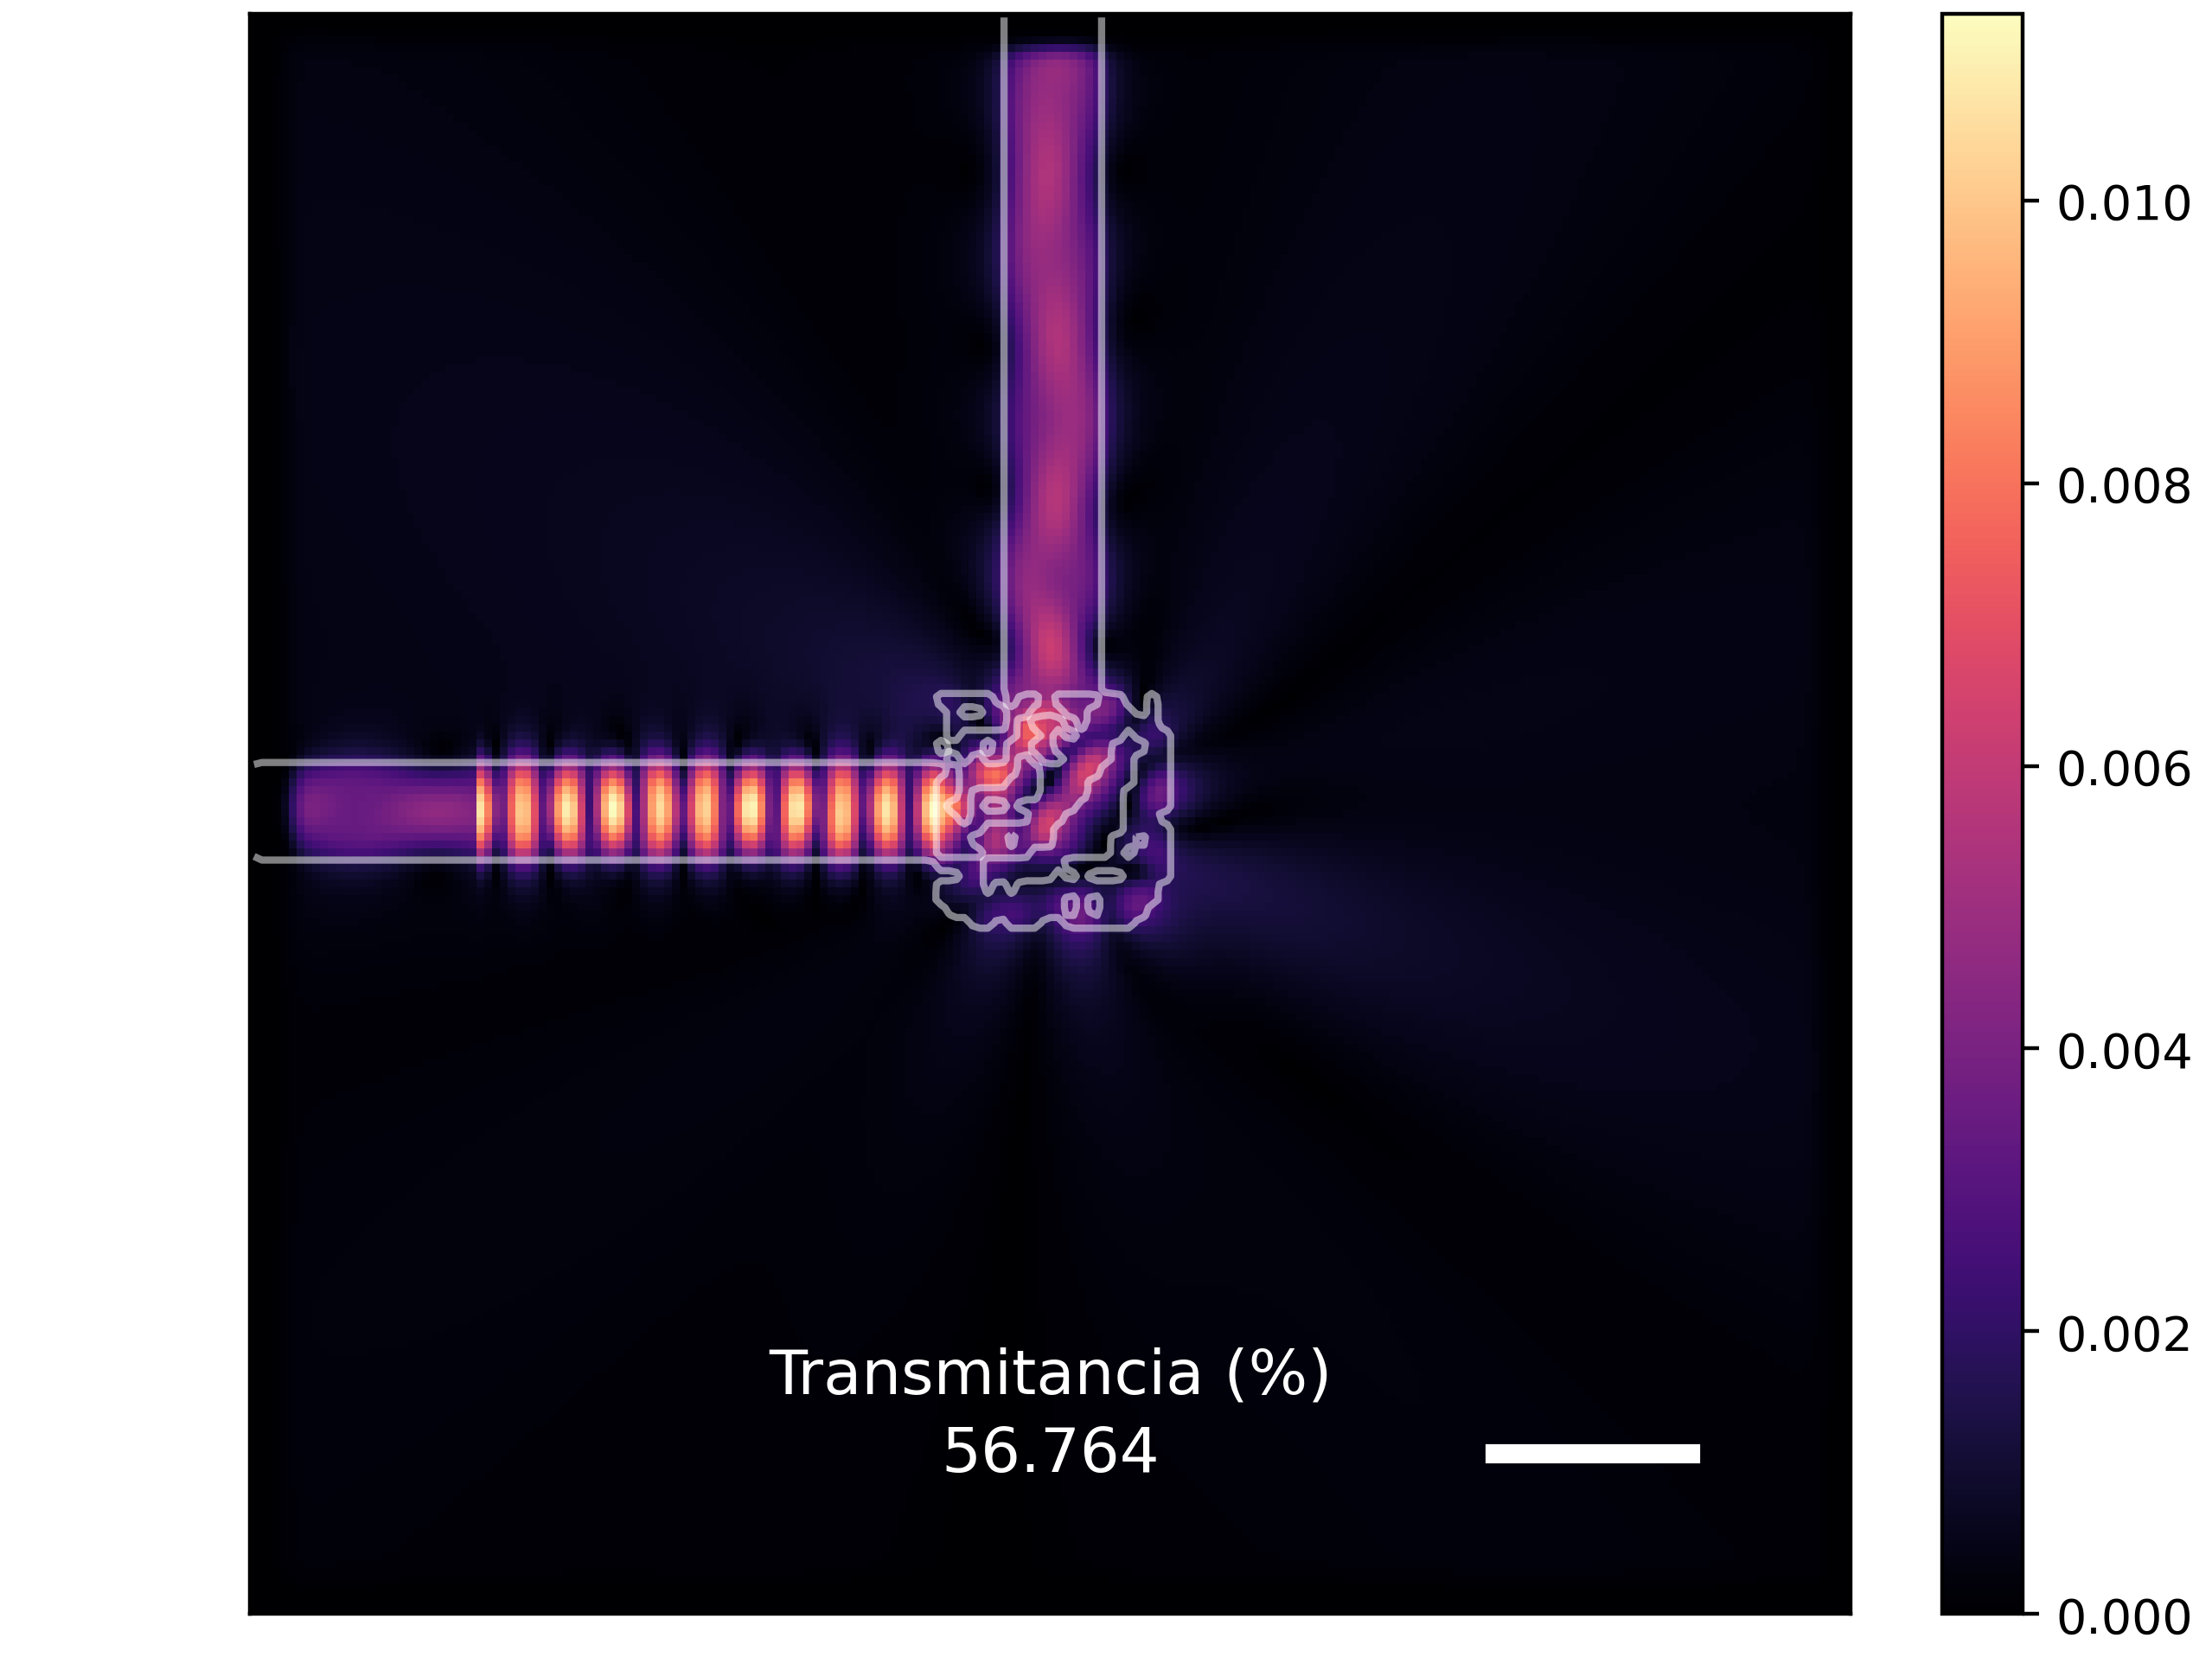
\includegraphics[width=0.80\textwidth]{image/results/device-v1-r40.png}
  \caption{Intensidad de campo eléctrico y transmitancia del diseño obtenidos en el experimento 1 simulado bajo una resolución de 40 $nm$. La línea blanca ubicada en la parte inferior derecha indica la escala de 1 $um$ en la figura.}
  \label{fig:exp1}
\end{figure}

En la figura \ref{fig:exp1} se muestra el diseño obtenido con este experimento, pero simulado con una resolución de $40 nm$.
Como se puede observar, hay una reducción a practicamente la mitad de la transmitancia que se estaba obteniendo al usar una resolución de $100 nm$.

\section{Experimento 2}

Con el anterior experimento se logró determinar la importancia de utilizar una adecuada resolución. Así, se procedió a trabajar con $40 nm$ de resolución.

\begin{figure}[ht]
  \centering
  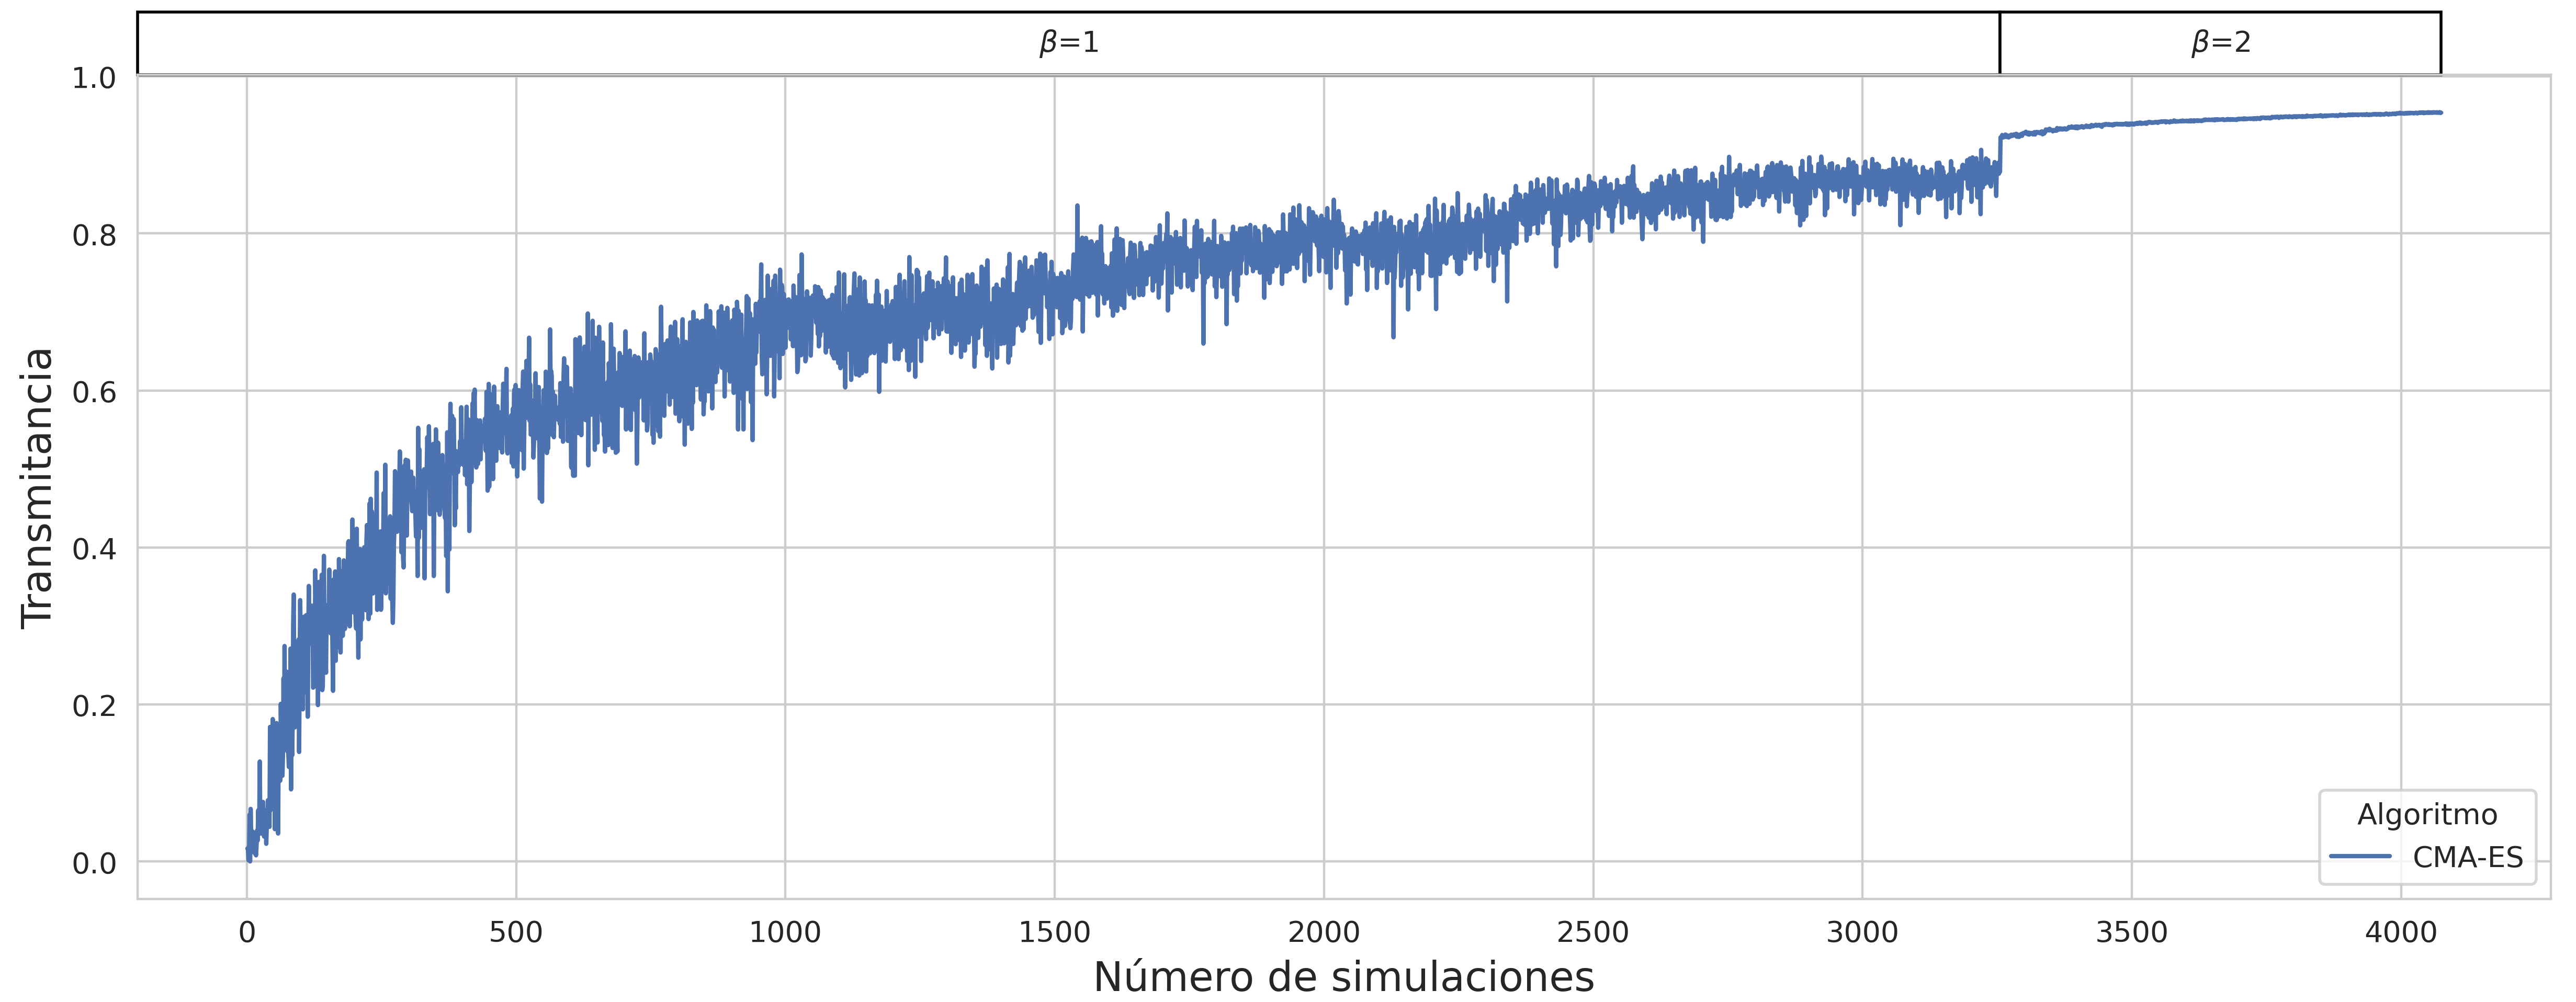
\includegraphics[width=\textwidth]{image/results/iterations_v2.png}
  \caption{Gráfica del número de simulaciones vs transmitancia producto de optimizar un \emph{bend} usando CMA-ES en el experimento 2.}
  \label{fig:iterations-v2}
\end{figure}


En total el experimento duró 4 días con 16 horas y en promedio cada simulación tomó 60.543 segundos.
Esto se debe al haber puesto la resolución en $40 nm$.

Como se puede observar en la figura \ref{fig:iterations-v2}, la optimización continua se realizó por alrededor de 3200 simulaciones y solo se avanzó un poco en la optimización discreta. Esto se debe al tiempo que estaba tomando la optimización. 
Sin embargo, aún cuando se realizaron menos simulaciones se obtuvieron mejores resultados que en el experimento 1 y con un mayor grado de confianza debido a la resolución usada.
En la figura \ref{fig:exp2-field-cont} se puede corroborar lo destacable de estos resultados.
Sin embargo, debido a la reducción en la cantidad de simulaciones, la optimización no logró llegar a fases con valores de $\beta$ mayores a 2, por ello los diseños aún no han convergido a valores reales.
Esto se puede apreciar en la figura $\ref{fig:exp2-eps-cont}$ donde las regiones grises representan la permitividad de un material no conocido.

\begin{figure}
  \centering
  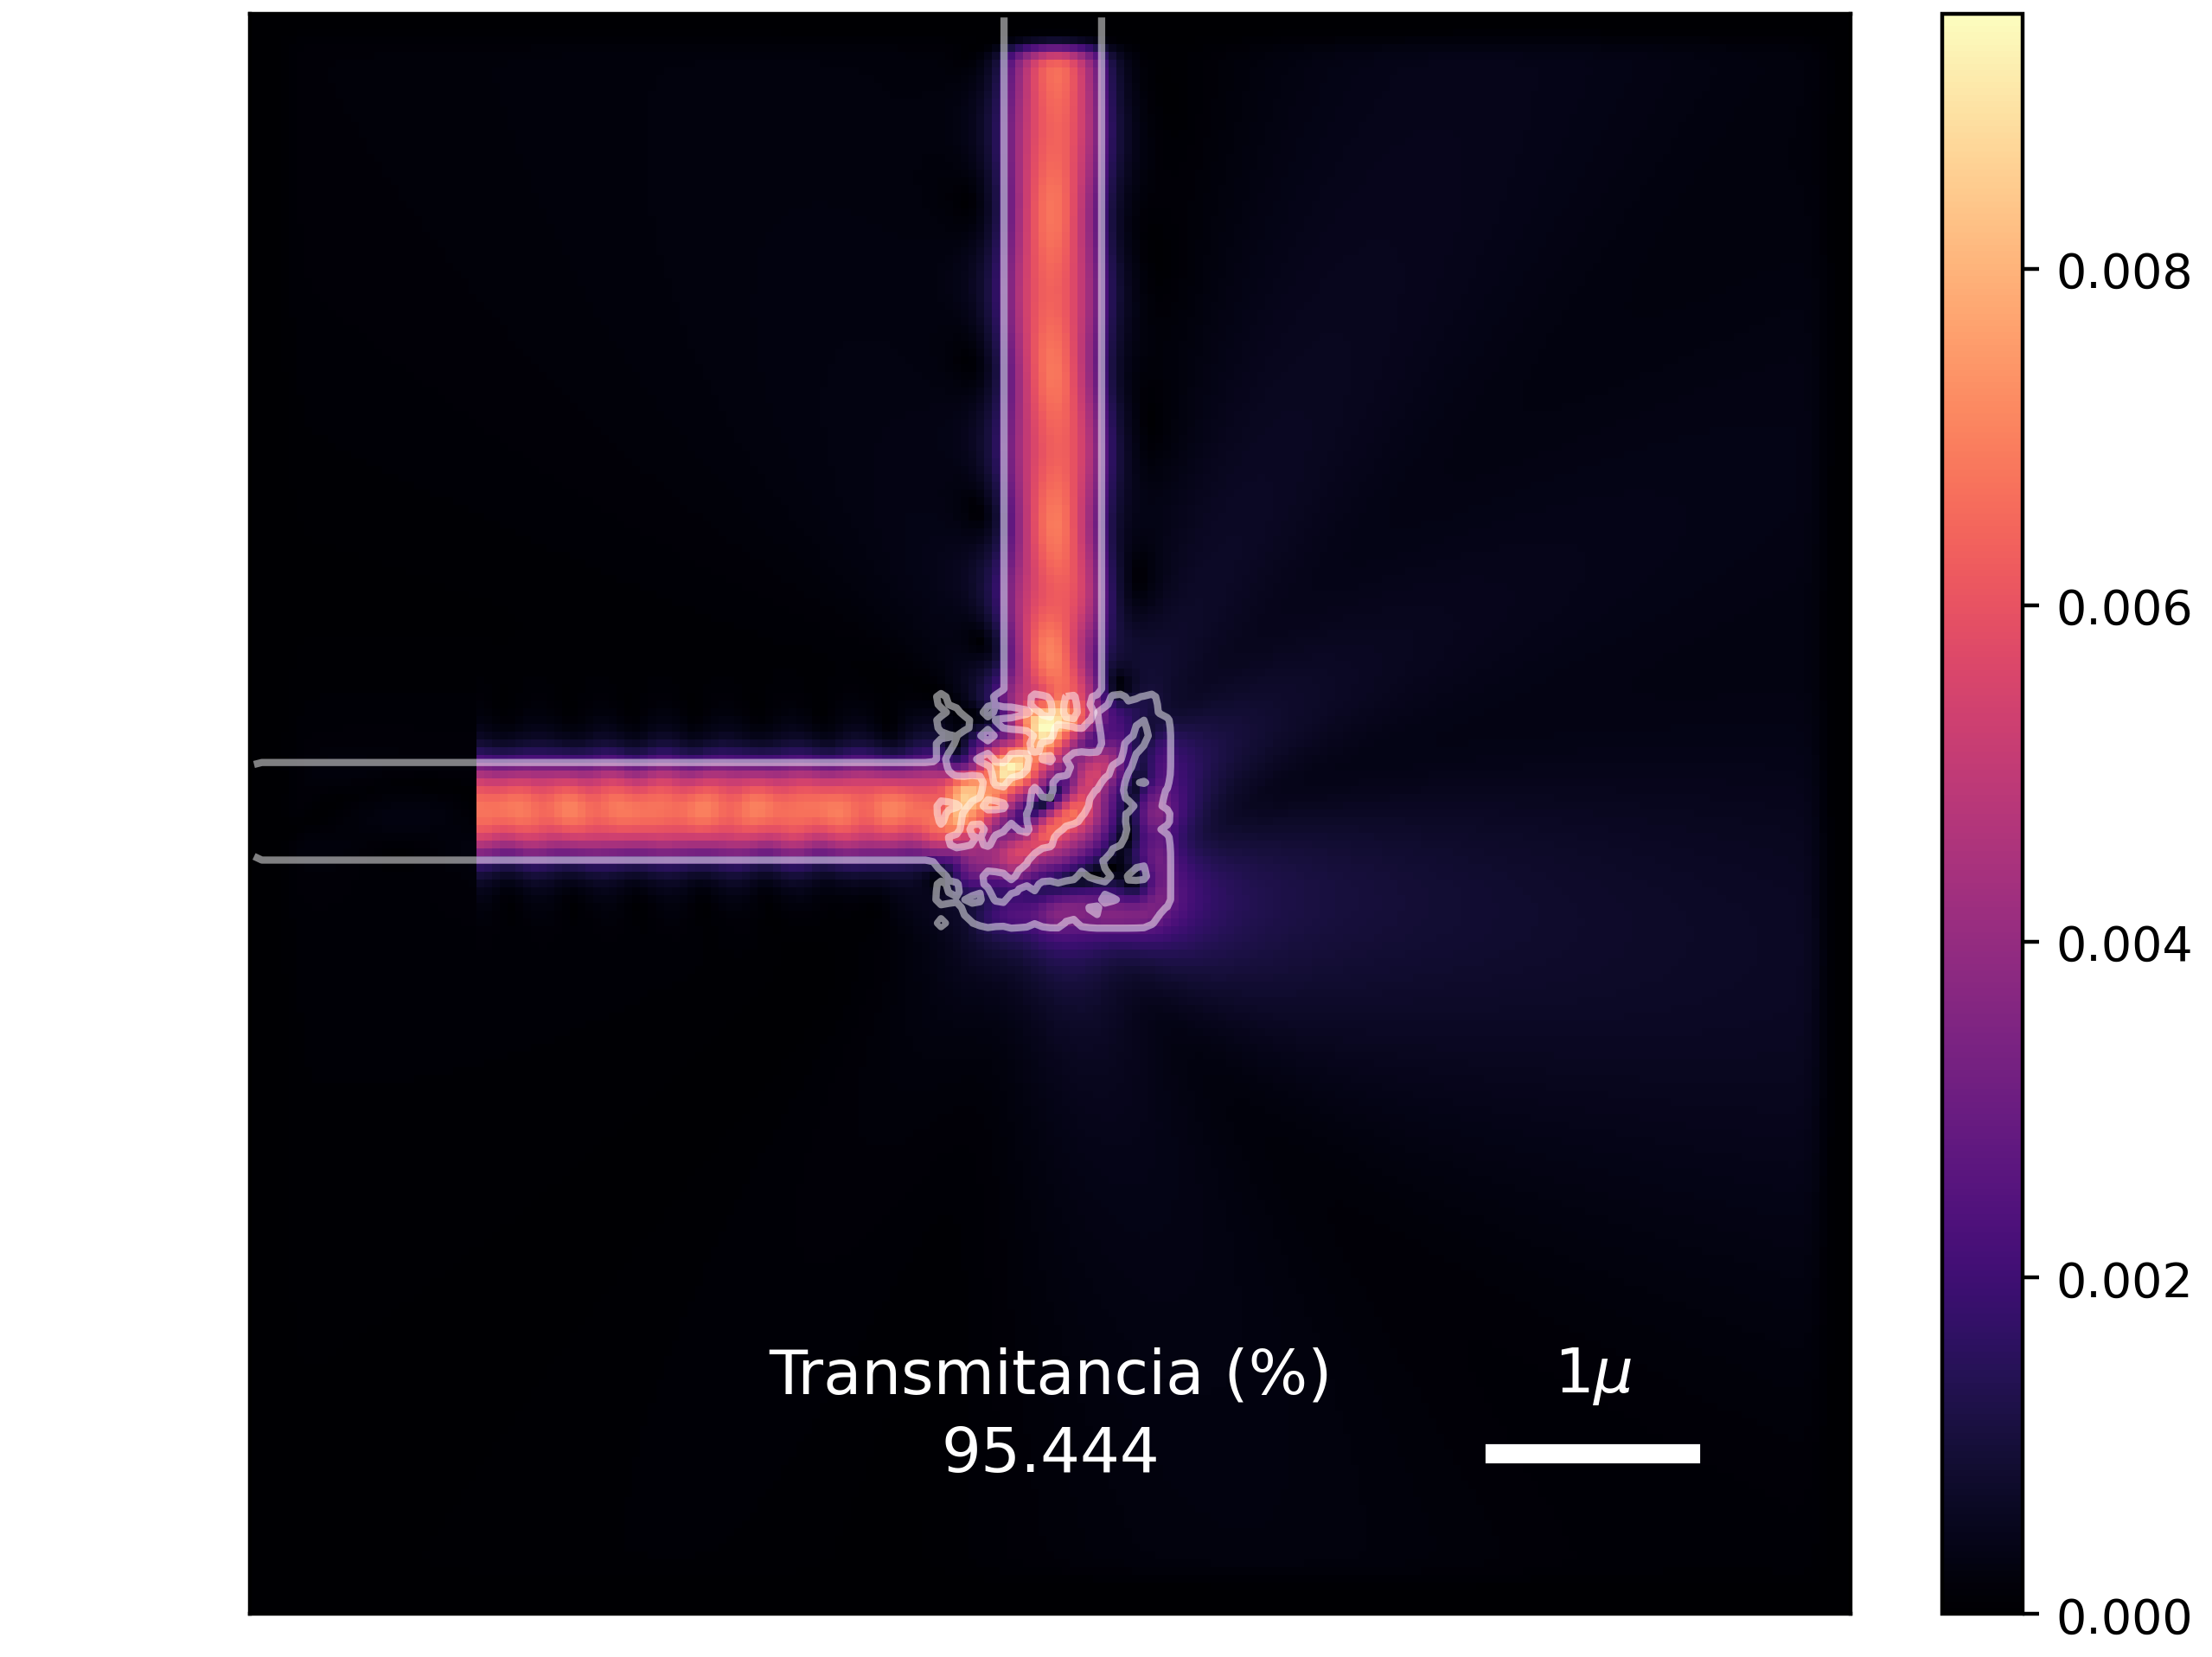
\includegraphics[width=0.80\textwidth]{image/results/device-v2-r40-cont.png}
  \caption{Intensidad de campo eléctrico y transmitancia del diseño obtenidos en el experimento 2 simulado bajo una resolución de 40 $nm$.}
  \label{fig:exp2-field-cont}
\end{figure}

\begin{figure}
  \centering
  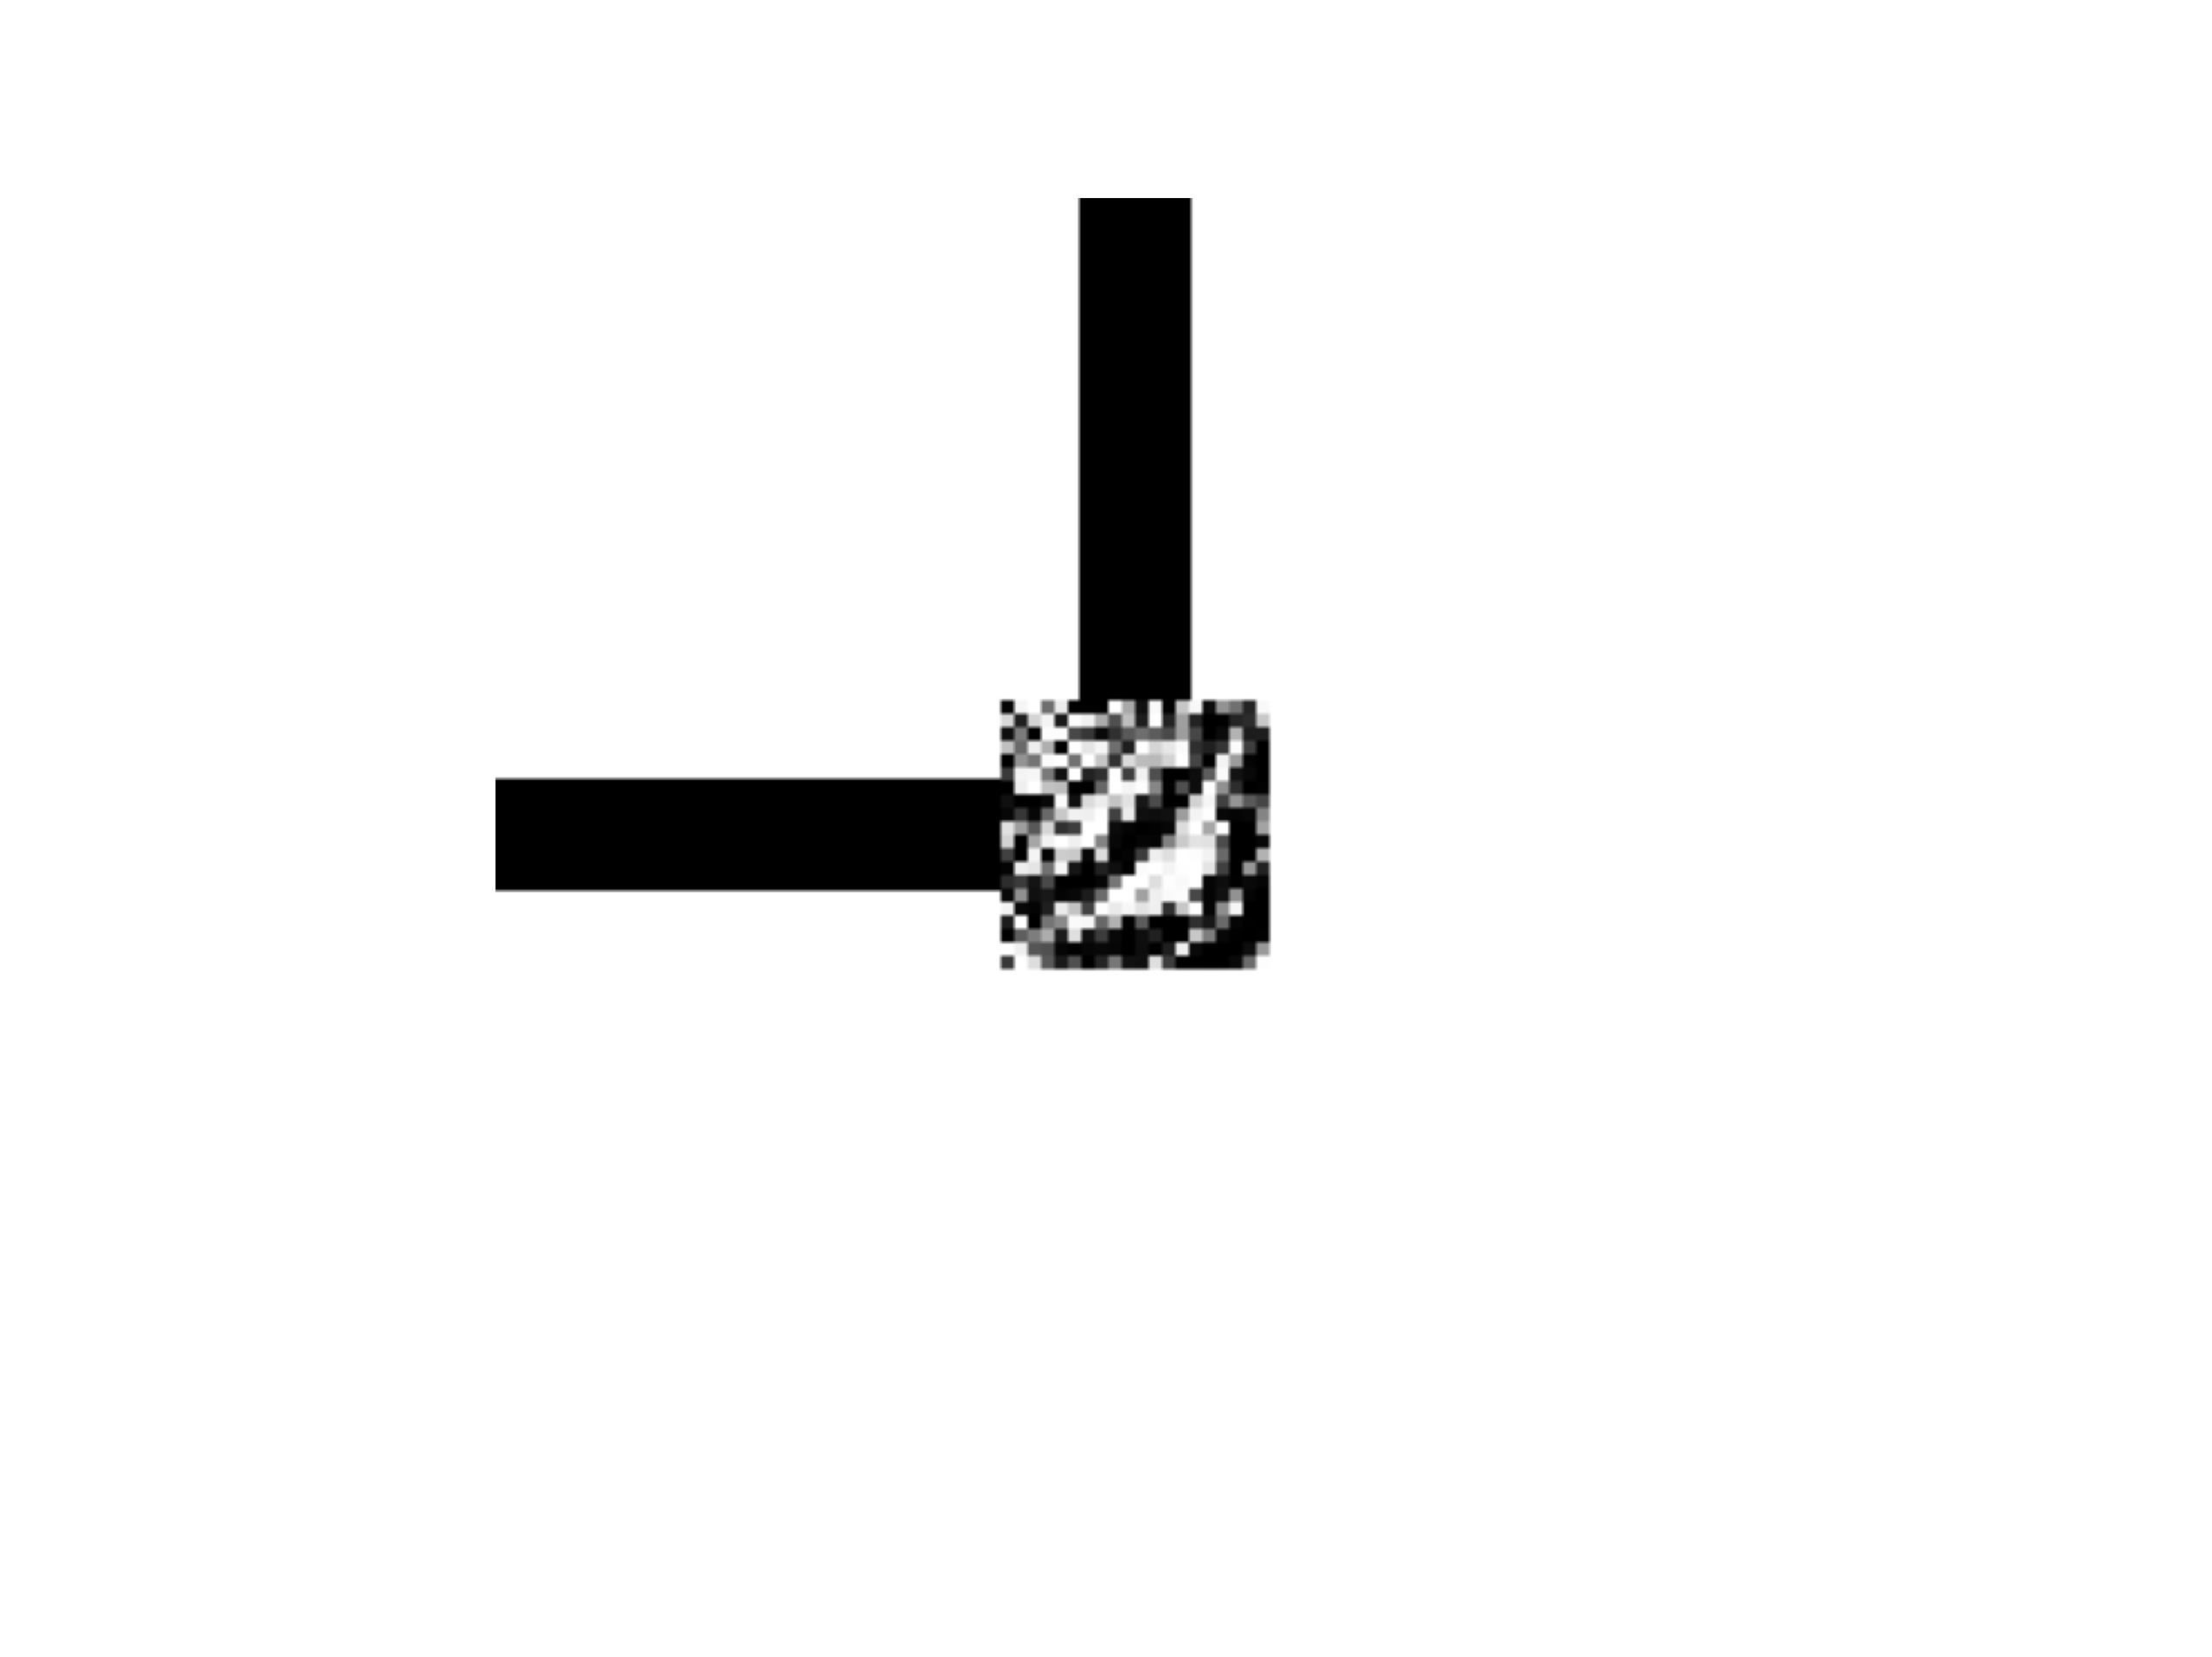
\includegraphics[width=0.60\textwidth]{image/results/eps-v2-cont.png}
  \caption{Distribución de la permitividad eléctrica del diseño del experimento 2.}
  \label{fig:exp2-eps-cont}
\end{figure}

Al resultado de este experimentó se le sometió a una discretización forzada (acercar la permitividad de cada píxel a la del $Si$ u $SiO_2$ de acuerdo a cual valor estuviera más cerca).
El diseño resultante se muestra en la figura \ref{fig:exp2-field-disc}, se observa que hay una reducción en el valor de la transmitancia.
A pesar de ello, los resultados son mejores que el experimento 1, esto nos lleva a suponer que de haber logrado ejecutarse la misma cantidad de iteraciones que en el experimento 1, se podría haber logrdo un dispositivo discretizado con una transmitancia alrededor del 95\%.

\begin{figure}
  \centering
  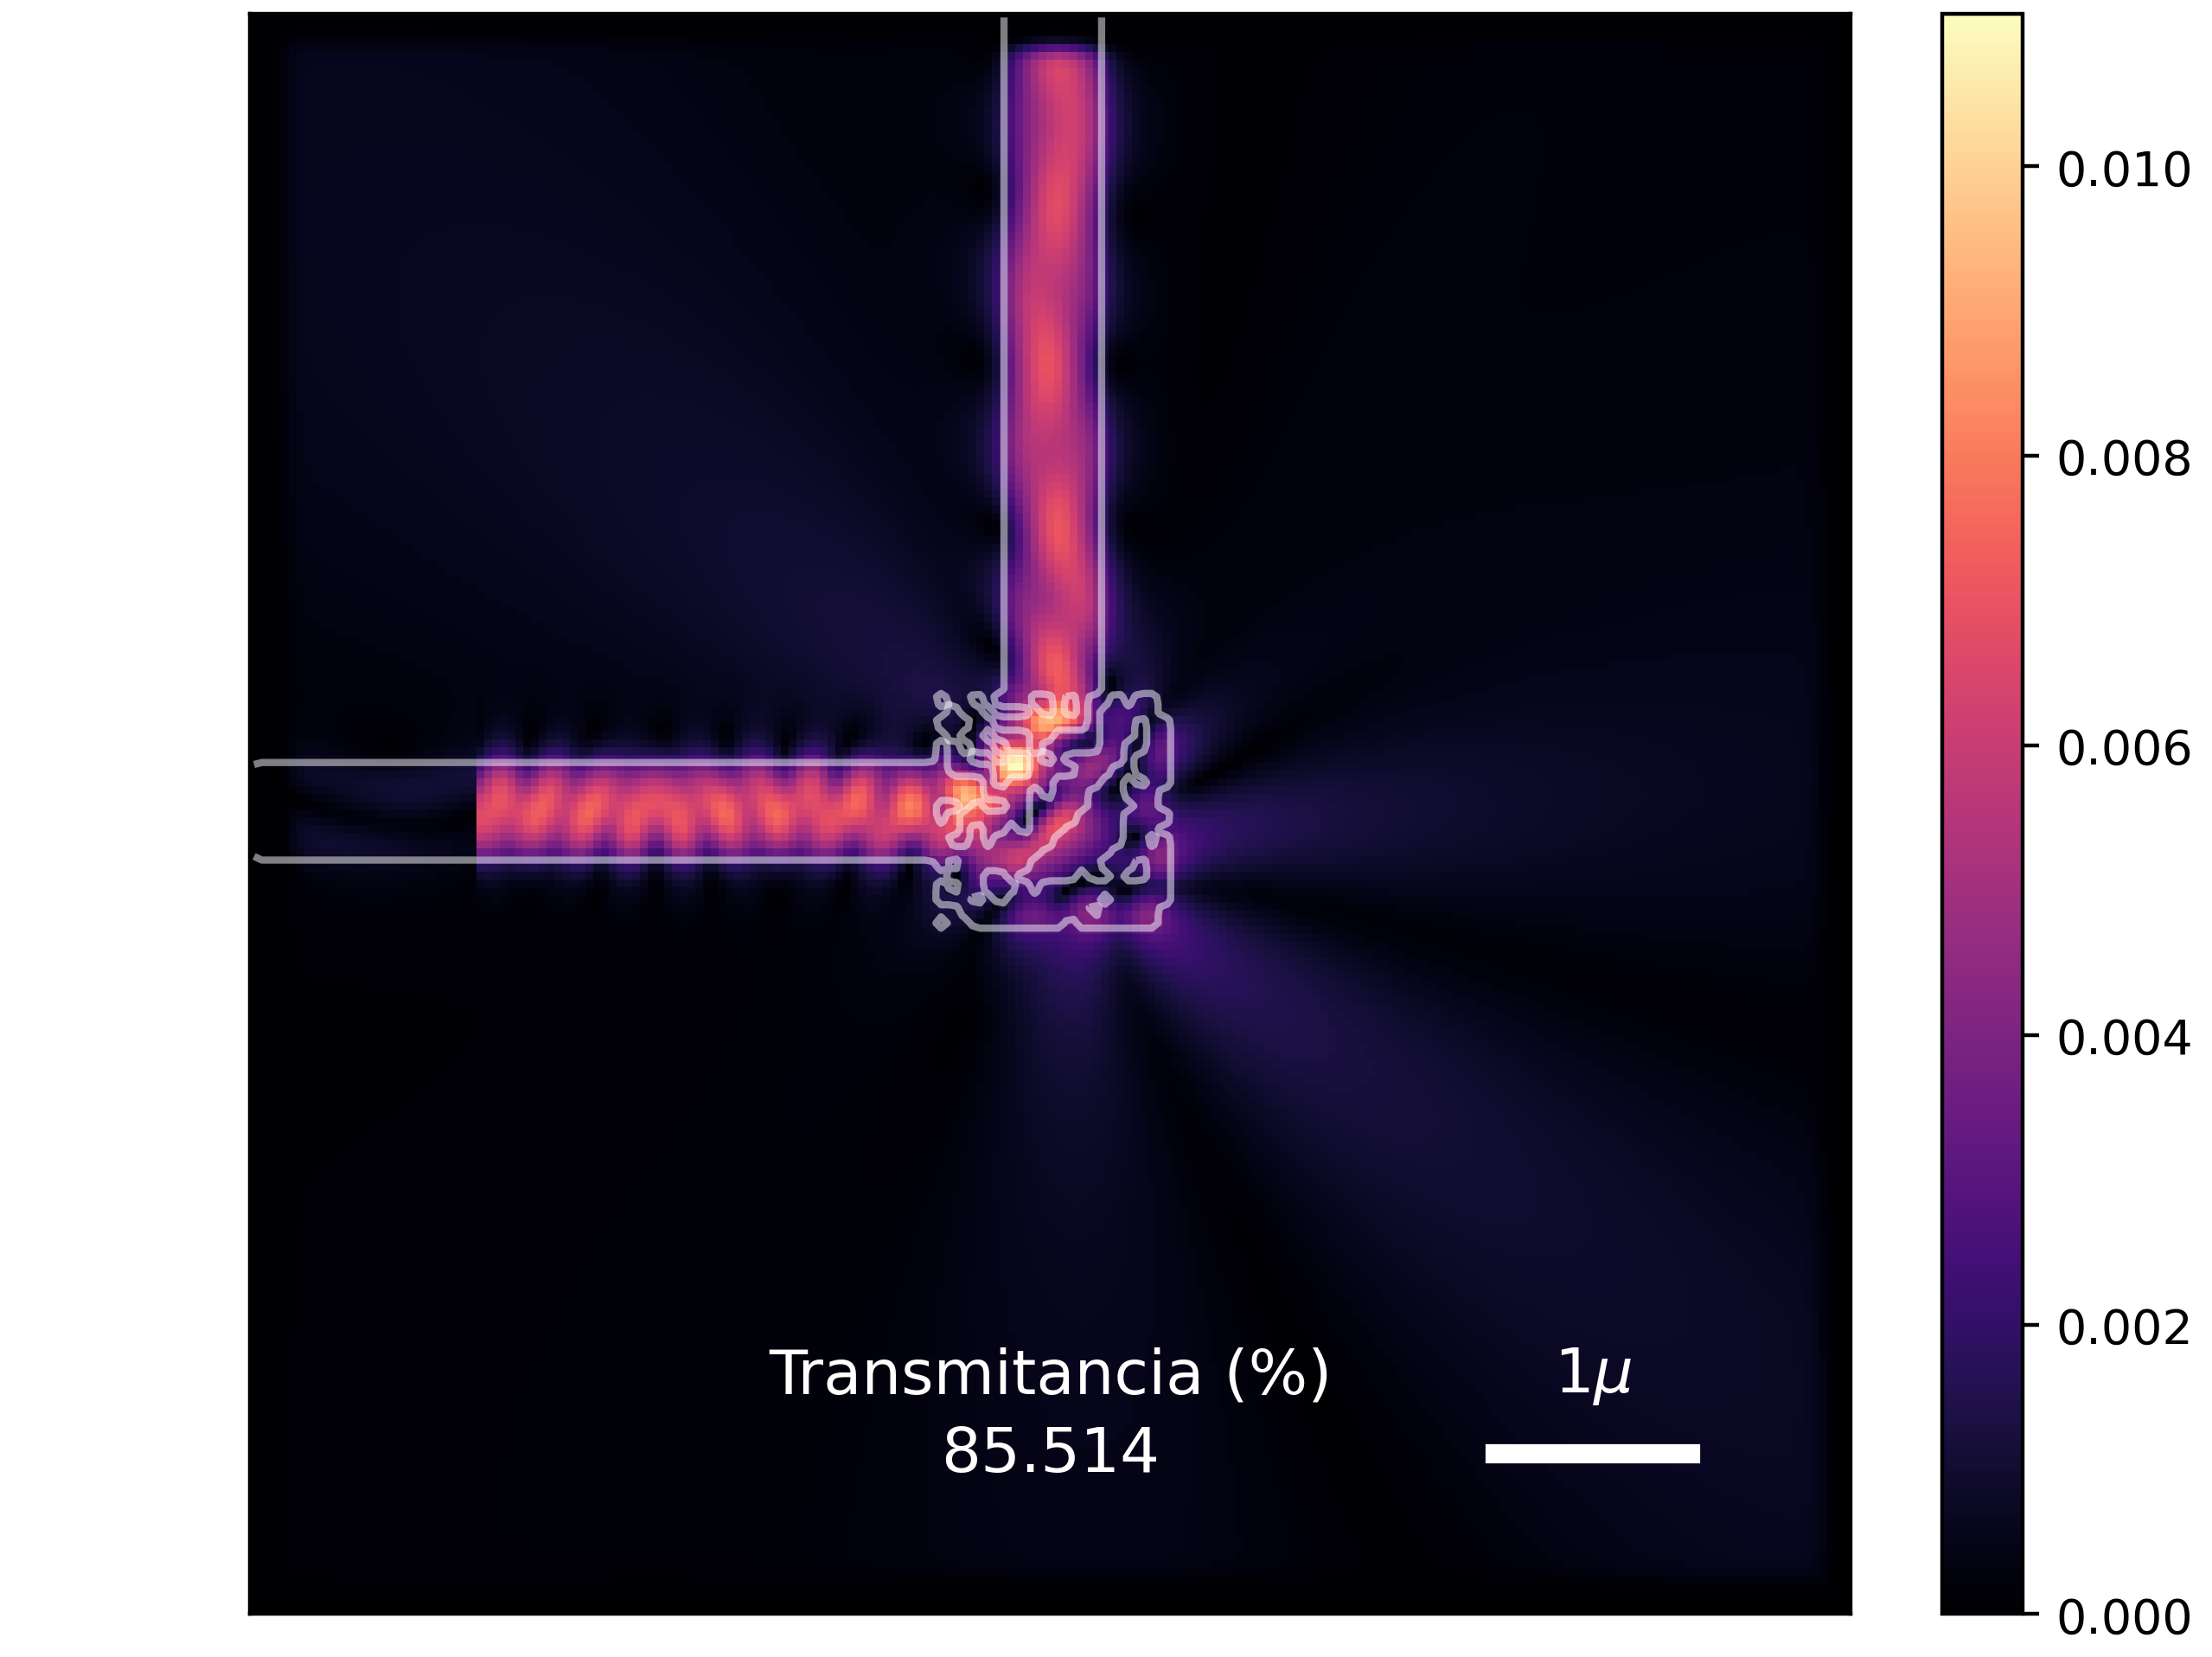
\includegraphics[width=0.80\textwidth]{image/results/device-v2-r40-disc.png}
  \caption{Intensidad de campo eléctrico y transmitancia del diseño obtenidos en el experimento 2 simulado bajo una resolución de 40 $nm$ tras ser discretizado.}
  \label{fig:exp2-field-disc}
\end{figure}


\section{Experimento 3}

Como tercer experimento se analizaron los resultados de las últimas evaluaciones realizadas en el anterior experimento.
Producto de ello, se encontró un diseño que ya estaba practicamente discretizado y que mantenía una transmitancia del 95.701 \%, además que presentaba curvas suaves que presumiblemente no tendrían dificultades para ser fabricadas. Este diseño se puede apreciar en la figura \ref{fig:exp3}.

\begin{figure}
  \centering
  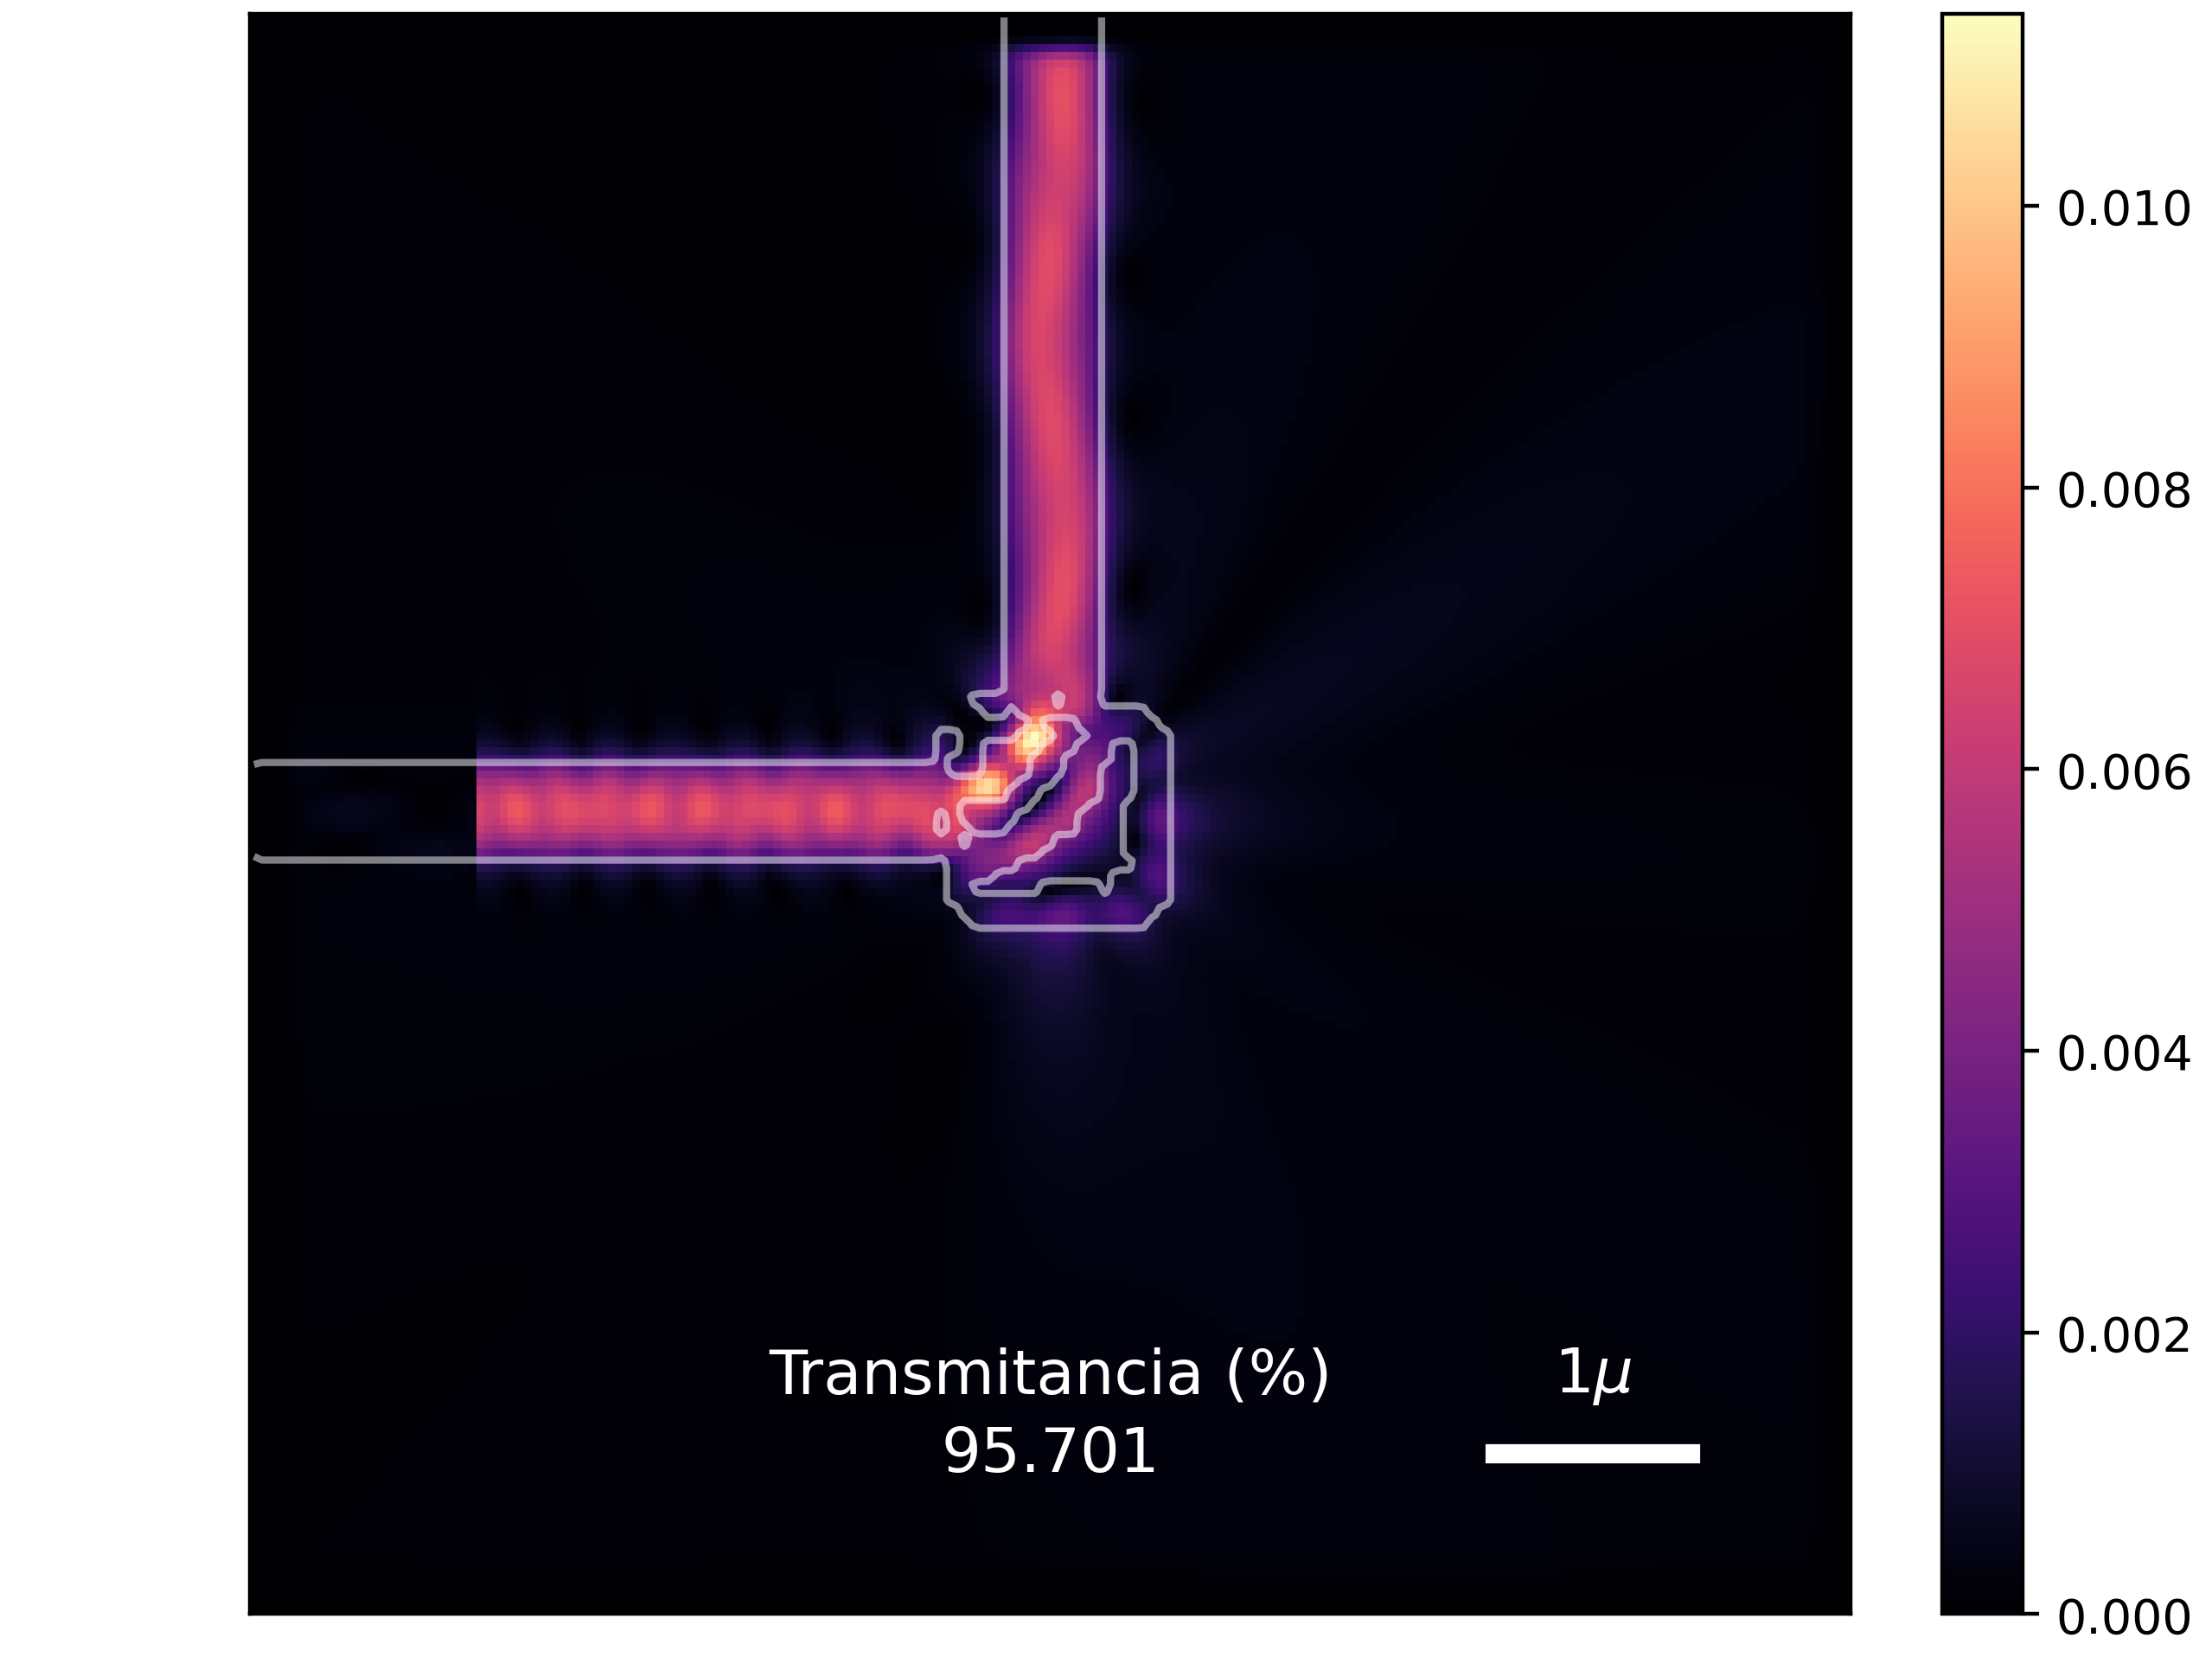
\includegraphics[width=0.80\textwidth]{image/results/device.png}
  \caption{Intensidad de campo eléctrico y transmitancia del diseño obtenidos en el experimento 3 simulado bajo una resolución de 40 $nm$.}
  \label{fig:exp3}
\end{figure}


A partir de los experimentos realizados se observa que se está logrando el objetivo de la tesis.
Cuando se logre completar las siguientes etapas de la metodología, principalmente las simulaciones en 3D y restricciones de fabricación, parece razonable el suponer que se obtendrán resultados favorables.
